% GNUPLOT: LaTeX picture with Postscript
\documentclass{minimal}
% Set font size
\makeatletter
\def\@ptsize{1}
\InputIfFileExists{size11.clo}{}{%
   \GenericError{(gnuplot) \space\space\space\@spaces}{%
      Gnuplot Error: File `size11.clo' not found! Could not set font size%
   }{See the gnuplot documentation for explanation.%
   }{For using a font size a file `size<fontsize>.clo' has to exist.
        Falling back ^^Jto default fontsize 10pt.}%
  \def\@ptsize{0}
  \input{size10.clo}%
}%
\makeatother
% Load packages
\usepackage{calc}
\usepackage{graphicx}
\usepackage{color}
\usepackage{transparent}
\makeatletter
% Select an appropriate default driver (from TeXLive graphics.cfg)
\begingroup
  \chardef\x=0 %
  % check pdfTeX
  \@ifundefined{pdfoutput}{}{%
    \ifcase\pdfoutput
    \else
      \chardef\x=1 %
    \fi
  }%
  % check VTeX
  \@ifundefined{OpMode}{}{%
    \chardef\x=2 %
  }%
\expandafter\endgroup
\ifcase\x
  % default case
  \PassOptionsToPackage{dvips}{geometry}
\or
  % pdfTeX is running in pdf mode
  \PassOptionsToPackage{pdftex}{geometry}
\else
  % VTeX is running
  \PassOptionsToPackage{vtex}{geometry}
\fi
\makeatother
% Set papersize
\usepackage[papersize={425.00bp,311.00bp},text={425.00bp,311.00bp}]{geometry}
% No page numbers and no paragraph indentation
\pagestyle{empty}
\setlength{\parindent}{0bp}%
% Load configuration file
\InputIfFileExists{gnuplot.cfg}{%
  \typeout{Using configuration file gnuplot.cfg}%
}{%
 \typeout{No configuration file gnuplot.cfg found.}%
}%
\renewcommand\familydefault{\sfdefault}\usepackage{cmbright}
\begin{document}
\begingroup
  \makeatletter
  \providecommand\color[2][]{%
    \GenericError{(gnuplot) \space\space\space\@spaces}{%
      Package color not loaded in conjunction with
      terminal option `colourtext'%
    }{See the gnuplot documentation for explanation.%
    }{Either use 'blacktext' in gnuplot or load the package
      color.sty in LaTeX.}%
    \renewcommand\color[2][]{}%
  }%
  \providecommand\includegraphics[2][]{%
    \GenericError{(gnuplot) \space\space\space\@spaces}{%
      Package graphicx or graphics not loaded%
    }{See the gnuplot documentation for explanation.%
    }{The gnuplot epslatex terminal needs graphicx.sty or graphics.sty.}%
    \renewcommand\includegraphics[2][]{}%
  }%
  \providecommand\rotatebox[2]{#2}%
  \@ifundefined{ifGPcolor}{%
    \newif\ifGPcolor
    \GPcolortrue
  }{}%
  \@ifundefined{ifGPblacktext}{%
    \newif\ifGPblacktext
    \GPblacktextfalse
  }{}%
  % define a \g@addto@macro without @ in the name:
  \let\gplgaddtomacro\g@addto@macro
  % define empty templates for all commands taking text:
  \gdef\gplbacktext{}%
  \gdef\gplfronttext{}%
  \makeatother
  \ifGPblacktext
    % no textcolor at all
    \def\colorrgb#1{}%
    \def\colorgray#1{}%
  \else
    % gray or color?
    \ifGPcolor
      \def\colorrgb#1{\color[rgb]{#1}}%
      \def\colorgray#1{\color[gray]{#1}}%
      \expandafter\def\csname LTw\endcsname{\color{white}}%
      \expandafter\def\csname LTb\endcsname{\color{black}}%
      \expandafter\def\csname LTa\endcsname{\color{black}}%
      \expandafter\def\csname LT0\endcsname{\color[rgb]{1,0,0}}%
      \expandafter\def\csname LT1\endcsname{\color[rgb]{0,1,0}}%
      \expandafter\def\csname LT2\endcsname{\color[rgb]{0,0,1}}%
      \expandafter\def\csname LT3\endcsname{\color[rgb]{1,0,1}}%
      \expandafter\def\csname LT4\endcsname{\color[rgb]{0,1,1}}%
      \expandafter\def\csname LT5\endcsname{\color[rgb]{1,1,0}}%
      \expandafter\def\csname LT6\endcsname{\color[rgb]{0,0,0}}%
      \expandafter\def\csname LT7\endcsname{\color[rgb]{1,0.3,0}}%
      \expandafter\def\csname LT8\endcsname{\color[rgb]{0.5,0.5,0.5}}%
    \else
      % gray
      \def\colorrgb#1{\color{black}}%
      \def\colorgray#1{\color[gray]{#1}}%
      \expandafter\def\csname LTw\endcsname{\color{white}}%
      \expandafter\def\csname LTb\endcsname{\color{black}}%
      \expandafter\def\csname LTa\endcsname{\color{black}}%
      \expandafter\def\csname LT0\endcsname{\color{black}}%
      \expandafter\def\csname LT1\endcsname{\color{black}}%
      \expandafter\def\csname LT2\endcsname{\color{black}}%
      \expandafter\def\csname LT3\endcsname{\color{black}}%
      \expandafter\def\csname LT4\endcsname{\color{black}}%
      \expandafter\def\csname LT5\endcsname{\color{black}}%
      \expandafter\def\csname LT6\endcsname{\color{black}}%
      \expandafter\def\csname LT7\endcsname{\color{black}}%
      \expandafter\def\csname LT8\endcsname{\color{black}}%
    \fi
  \fi
    \setlength{\unitlength}{0.0500bp}%
    \ifx\gptboxheight\undefined%
      \newlength{\gptboxheight}%
      \newlength{\gptboxwidth}%
      \newsavebox{\gptboxtext}%
    \fi%
    \setlength{\fboxrule}{0.5pt}%
    \setlength{\fboxsep}{1pt}%
\begin{picture}(8500.00,6220.00)%
    \gplgaddtomacro\gplbacktext{%
      \csname LTb\endcsname%%
      \put(724,4146){\makebox(0,0)[r]{\strut{}$0$}}%
      \csname LTb\endcsname%%
      \put(724,4523){\makebox(0,0)[r]{\strut{}$0.2$}}%
      \csname LTb\endcsname%%
      \put(724,4901){\makebox(0,0)[r]{\strut{}$0.4$}}%
      \csname LTb\endcsname%%
      \put(724,5278){\makebox(0,0)[r]{\strut{}$0.6$}}%
      \csname LTb\endcsname%%
      \put(724,5656){\makebox(0,0)[r]{\strut{}$0.8$}}%
      \csname LTb\endcsname%%
      \put(724,6033){\makebox(0,0)[r]{\strut{}$1$}}%
    }%
    \gplgaddtomacro\gplfronttext{%
      \csname LTb\endcsname%%
      \put(232,5089){\rotatebox{-270}{\makebox(0,0){\strut{}$y / \mathcal{L}$}}}%
      \csname LTb\endcsname%%
      \put(4486,4600){\makebox(0,0)[l]{\strut{}$-5$}}%
      \csname LTb\endcsname%%
      \put(4486,5176){\makebox(0,0)[l]{\strut{}$-3$}}%
      \csname LTb\endcsname%%
      \put(4486,5752){\makebox(0,0)[l]{\strut{}$-1$}}%
      \csname LTb\endcsname%%
      \put(4894,5089){\rotatebox{-270}{\makebox(0,0){\strut{}$U / \epsilon$}}}%
      \colorrgb{0.87,0.09,0.12}%%
      \put(2978,5750){\makebox(0,0)[l]{\strut{}f}}%
    }%
    \gplgaddtomacro\gplbacktext{%
      \csname LTb\endcsname%%
      \put(714,558){\makebox(0,0)[r]{\strut{}$0$}}%
      \csname LTb\endcsname%%
      \put(714,848){\makebox(0,0)[r]{\strut{}$0.05$}}%
      \csname LTb\endcsname%%
      \put(714,1137){\makebox(0,0)[r]{\strut{}$0.1$}}%
      \csname LTb\endcsname%%
      \put(714,1427){\makebox(0,0)[r]{\strut{}$0.15$}}%
      \csname LTb\endcsname%%
      \put(714,1716){\makebox(0,0)[r]{\strut{}$0.2$}}%
      \csname LTb\endcsname%%
      \put(714,2006){\makebox(0,0)[r]{\strut{}$0.25$}}%
      \csname LTb\endcsname%%
      \put(714,2295){\makebox(0,0)[r]{\strut{}$0.3$}}%
      \csname LTb\endcsname%%
      \put(816,372){\makebox(0,0){\strut{}$0$}}%
      \csname LTb\endcsname%%
      \put(1371,372){\makebox(0,0){\strut{}$0.5$}}%
      \csname LTb\endcsname%%
      \put(1926,372){\makebox(0,0){\strut{}$1$}}%
      \csname LTb\endcsname%%
      \put(2482,372){\makebox(0,0){\strut{}$1.5$}}%
      \csname LTb\endcsname%%
      \put(3037,372){\makebox(0,0){\strut{}$2$}}%
      \csname LTb\endcsname%%
      \put(3592,372){\makebox(0,0){\strut{}$2.5$}}%
      \csname LTb\endcsname%%
      \put(4147,372){\makebox(0,0){\strut{}$3$}}%
    }%
    \gplgaddtomacro\gplfronttext{%
      \csname LTb\endcsname%%
      \put(120,1513){\rotatebox{-270}{\makebox(0,0){\strut{}$p_s$}}}%
      \csname LTb\endcsname%%
      \put(2481,93){\makebox(0,0){\strut{}$x / \mathcal{L}$}}%
    }%
    \gplgaddtomacro\gplbacktext{%
      \csname LTb\endcsname%%
      \put(714,2749){\makebox(0,0)[r]{\strut{}$-4$}}%
      \csname LTb\endcsname%%
      \put(714,3234){\makebox(0,0)[r]{\strut{}$-2$}}%
      \csname LTb\endcsname%%
      \put(714,3718){\makebox(0,0)[r]{\strut{}$0$}}%
      \csname LTb\endcsname%%
      \put(816,2321){\makebox(0,0){\strut{}}}%
      \csname LTb\endcsname%%
      \put(1371,2321){\makebox(0,0){\strut{}}}%
      \csname LTb\endcsname%%
      \put(1926,2321){\makebox(0,0){\strut{}}}%
      \csname LTb\endcsname%%
      \put(2482,2321){\makebox(0,0){\strut{}}}%
      \csname LTb\endcsname%%
      \put(3037,2321){\makebox(0,0){\strut{}}}%
      \csname LTb\endcsname%%
      \put(3592,2321){\makebox(0,0){\strut{}}}%
      \csname LTb\endcsname%%
      \put(4147,2321){\makebox(0,0){\strut{}}}%
      \csname LTb\endcsname%%
      \put(85,3918){\makebox(0,0)[l]{\strut{}(b)}}%
      \csname LTb\endcsname%%
      \put(4334,3918){\makebox(0,0)[l]{\strut{}(c)}}%
      \csname LTb\endcsname%%
      \put(85,2425){\makebox(0,0)[l]{\strut{}(d)}}%
    }%
    \gplgaddtomacro\gplfronttext{%
      \csname LTb\endcsname%%
      \put(324,3233){\rotatebox{-270}{\makebox(0,0){\strut{}$U~/\epsilon$}}}%
      \csname LTb\endcsname%%
      \put(1316,3476){\makebox(0,0)[l]{\strut{}$A$}}%
      \csname LTb\endcsname%%
      \put(2426,3112){\makebox(0,0)[l]{\strut{}$B$}}%
      \csname LTb\endcsname%%
      \put(3536,2749){\makebox(0,0)[l]{\strut{}$C$}}%
      \colorrgb{0.87,0.09,0.12}%%
      \put(1460,3016){\makebox(0,0)[l]{\strut{}f}}%
      \csname LTb\endcsname%%
      \put(85,5970){\makebox(0,0)[l]{\strut{}(a)}}%
    }%
    \gplgaddtomacro\gplbacktext{%
      \csname LTb\endcsname%%
      \put(4964,578){\makebox(0,0)[r]{\strut{}$0$}}%
      \csname LTb\endcsname%%
      \put(4964,1197){\makebox(0,0)[r]{\strut{}$0.02$}}%
      \csname LTb\endcsname%%
      \put(4964,1815){\makebox(0,0)[r]{\strut{}$0.04$}}%
      \csname LTb\endcsname%%
      \put(4964,2434){\makebox(0,0)[r]{\strut{}$0.06$}}%
      \csname LTb\endcsname%%
      \put(4964,3053){\makebox(0,0)[r]{\strut{}$0.08$}}%
      \csname LTb\endcsname%%
      \put(4964,3672){\makebox(0,0)[r]{\strut{}$0.1$}}%
      \csname LTb\endcsname%%
      \put(5066,392){\makebox(0,0){\strut{}$1$}}%
      \csname LTb\endcsname%%
      \put(6120,392){\makebox(0,0){\strut{}$10$}}%
      \csname LTb\endcsname%%
      \put(7173,392){\makebox(0,0){\strut{}$100$}}%
      \csname LTb\endcsname%%
      \put(8227,392){\makebox(0,0){\strut{}$1000$}}%
      \csname LTb\endcsname%%
      \put(85,3918){\makebox(0,0)[l]{\strut{}(b)}}%
      \csname LTb\endcsname%%
      \put(4334,3918){\makebox(0,0)[l]{\strut{}(c)}}%
      \csname LTb\endcsname%%
      \put(85,2425){\makebox(0,0)[l]{\strut{}(d)}}%
    }%
    \gplgaddtomacro\gplfronttext{%
      \csname LTb\endcsname%%
      \put(4370,2279){\rotatebox{-270}{\makebox(0,0){\strut{}$p_{\; \textrm{FPT}}$}}}%
      \csname LTb\endcsname%%
      \put(6646,113){\makebox(0,0){\strut{}$t / \tau$}}%
      \csname LTb\endcsname%%
      \put(7813,5628){\makebox(0,0)[r]{\strut{}Rew 1D$: f=9~\epsilon / \mathcal{L} \rightarrow f=0$}}%
      \csname LTb\endcsname%%
      \put(7813,5442){\makebox(0,0)[r]{\strut{}Rew 1D$: f=0 \rightarrow f=9~\epsilon / \mathcal{L}$}}%
      \csname LTb\endcsname%%
      \put(7813,5256){\makebox(0,0)[r]{\strut{}Simulation 1D$: f=0~\epsilon / \mathcal{L}$}}%
      \csname LTb\endcsname%%
      \put(7813,5070){\makebox(0,0)[r]{\strut{}Simulation 1D$: f=9~\epsilon / \mathcal{L}$}}%
      \csname LTb\endcsname%%
      \put(7813,4884){\makebox(0,0)[r]{\strut{}Rew 2D$: f=9~\epsilon / \mathcal{L} \rightarrow f=0$}}%
      \csname LTb\endcsname%%
      \put(7813,4698){\makebox(0,0)[r]{\strut{}Rew 2D$: f=0 \rightarrow f=9~\epsilon / \mathcal{L}$}}%
      \csname LTb\endcsname%%
      \put(7813,4512){\makebox(0,0)[r]{\strut{}Simulation 2D$: f=0~\epsilon / \mathcal{L}$}}%
      \csname LTb\endcsname%%
      \put(7813,4326){\makebox(0,0)[r]{\strut{}Simulation 2D$: f=9~\epsilon / \mathcal{L}$}}%
      \csname LTb\endcsname%%
      \put(85,5970){\makebox(0,0)[l]{\strut{}(a)}}%
    }%
    \gplbacktext
    \put(0,0){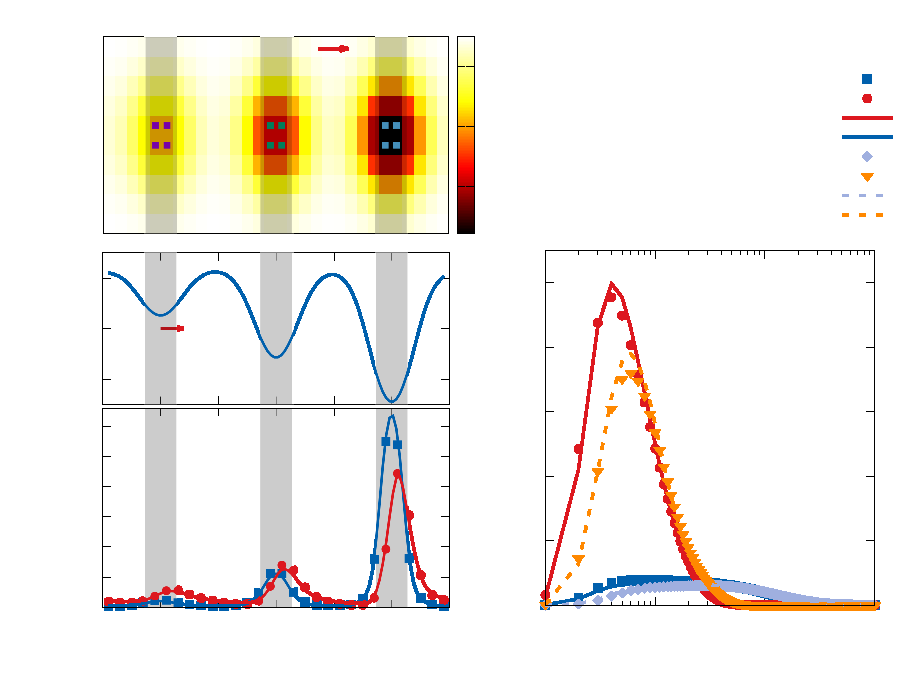
\includegraphics{single_1030-inc}}%
    \gplfronttext
  \end{picture}%
\endgroup
\end{document}
